\section{Design}
    \subsection{Sequence Diagrams}
        \subsubsection{View Map}
            \begin{figure}[H]
                \centering
                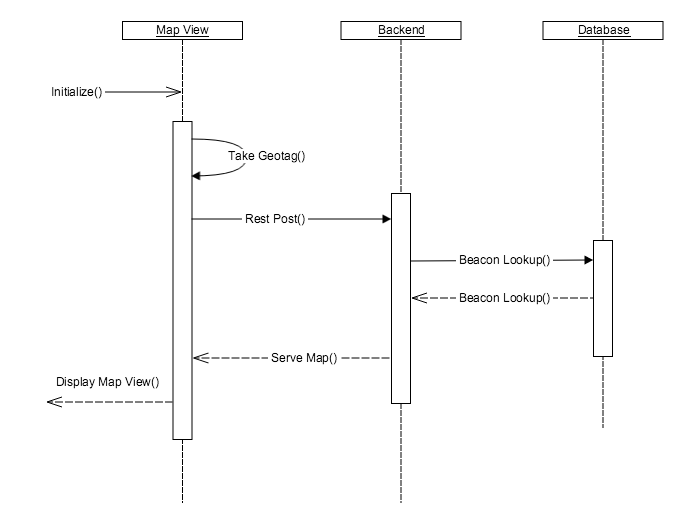
\includegraphics[width=\textwidth]{src/img/view-map.png}
                \caption{View Map Sequence Diagram} 
            \end{figure}

            Map View will initialize when the app opens or when the user chooses
            to view the map. Upon initialization, a geotag of the current
            location is taken. The backend is then sent a Rest post with the
            geotag data. The backend polls the database to lookup nearby
            beacons. The database returns the nearby beacons. The backend serves
            the beacon data to Map View and the map is displayed. 

        \subsubsection{Post Beacon}
            \begin{figure}[H]
                \centering
                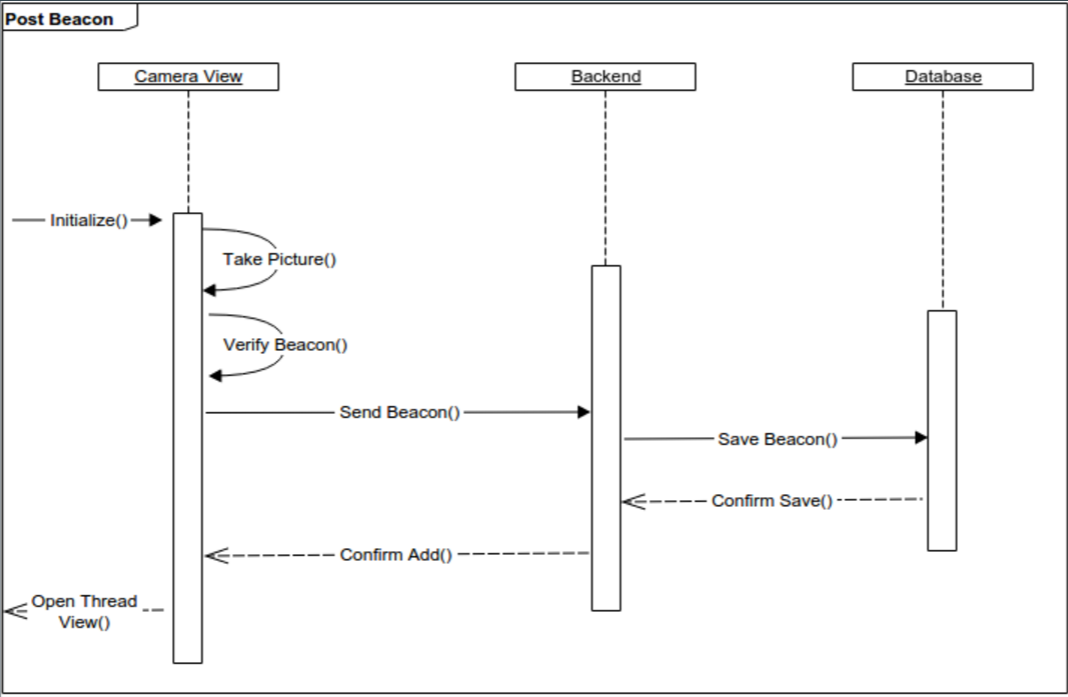
\includegraphics[width=\textwidth]{src/img/post-beacon.png}
                \caption{Post Beacon Sequence Diagram} 
            \end{figure}

            From Camera View, the user will take a picture, verify the picture
            and optionally add a text description of the picture. A geotag of
            the current location is also taken. Camera View will take the new
            picture, text, and geotag and format it into a Rest post and send
            the data to the backend. The backend will poll the database to
            create and save the new beacon. Once the database has saved the
            beacon, a confirmation is returned. The backend then returns a
            success message to the user. The new beacon is also opened in thread
            view for the user. 

        \subsubsection{View Thread}
            \begin{figure}[H]
                \centering
                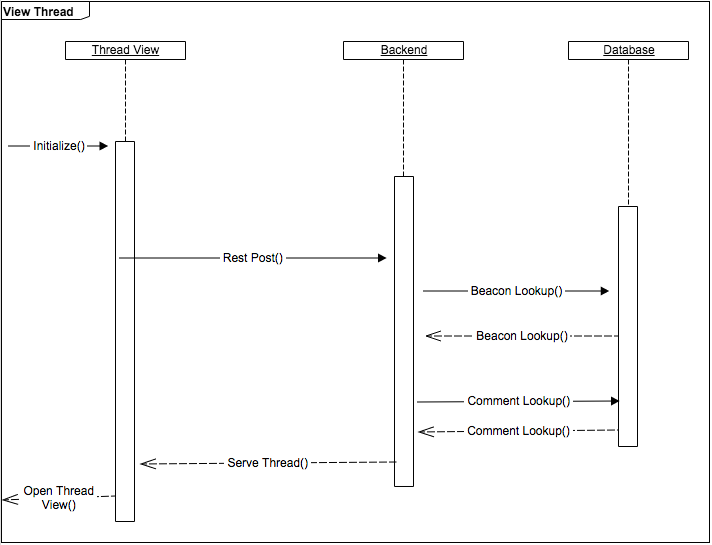
\includegraphics[width=\textwidth]{src/img/view-thread.png}
                \caption{View Thread Sequence Diagram} 
            \end{figure}

            Thread View is opened after posting a new beacon or when a beacon is
            otherwise selected. A Rest post is sent to the backend to notify the
            backend which beacon needs to be found via Post ID. The backend
            polls the database to lookup the beacon. Once found the database
            returns the beacon data to the backend. The backend then polls the
            database for the corresponding comments. The comments are returned
            to the backend. The backend bundles the beacon and comments together
            and serves them to Thread View. Thread View then displays to the
            user. 

        \subsubsection{Heart Post}
            \begin{figure}[H]
                \centering
                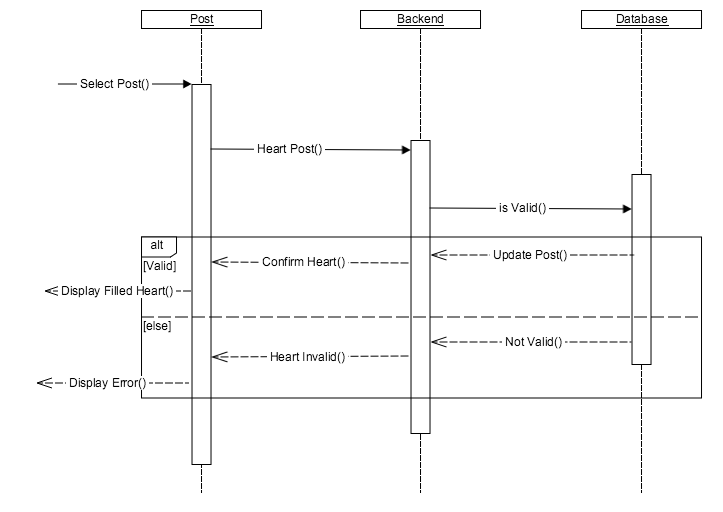
\includegraphics[width=\textwidth]{src/img/heart-post.png}
                \caption{Heart Post Sequence Diagram} 
            \end{figure}

            From thread view or while viewing a beacon thumbnail, a user may
            select a heart icon to heart the corresponding post. The request is
            sent to the backend via a Rest post. The backend polls the database
            to determine if the post is able to be hearted by that user. If the
            request is valid the database updates the post and returns success
            to the backend. The backend confirms the action of hearting to the
            selected post. The heart is then shown to be filled to the user. If
            the request to heart is invalid, the database returns an error. The
            backend serves the post with an error, and the user is notified that
            the action was not valid. These steps are the same for hearting and
            unhearting a post, but there will be separate URIs. 

        \subsubsection{Post Comment}
            \begin{figure}[H]
                \centering
                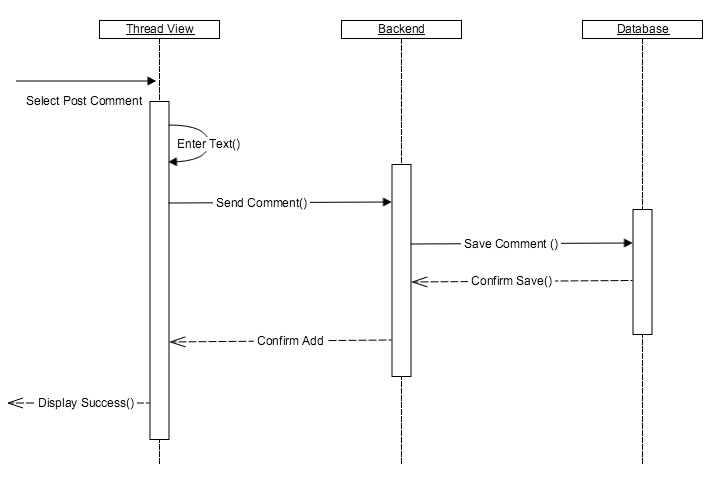
\includegraphics[width=\textwidth]{src/img/post-comment.png}
                \caption{Post Comment Sequence Diagram} 
            \end{figure}

            From Thread View, may choose to post a comment. They will then be
            prompted to enter text as the body of the new comment. The text is
            sent to the backend along with the user ID via REST post. The
            backend sends the data to the database to be saved. Upon saving of
            the comment, the database returns a confirmation to the backend. The
            backend notifies Thread View that the comment was successfully
            added. Thread View displays a success message to the user.

        \subsubsection{View User}
            \begin{figure}[H]
                \centering
                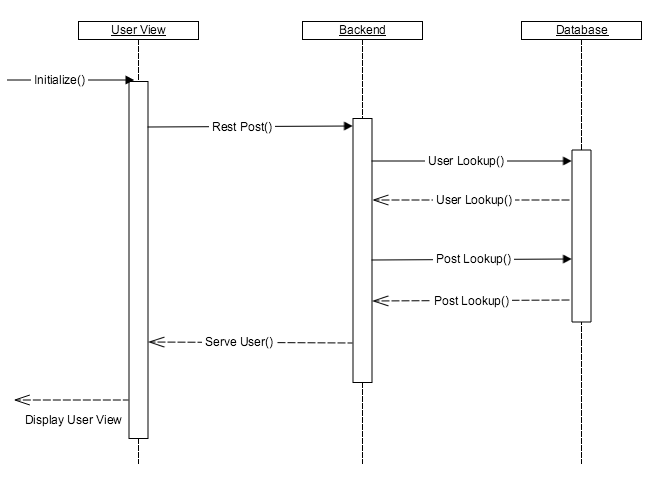
\includegraphics[width=\textwidth]{src/img/view-user.png}
                \caption{View User Sequence Diagram} 
            \end{figure}

            Profile View is opened when a user selects to see a user’s profile.
            A REST post is sent to the backend with the user ID of the user
            being viewed. The backend polls the database to lookup the user. The
            database returns the user data. The backend then polls the database
            for the user’s posts. The database returns the user’s posts. The
            backend then serves Profile view with the user and post data.
            Profile view is displayed to the user. 

        \subsubsection{Follow User}
            \begin{figure}[H]
                \centering
                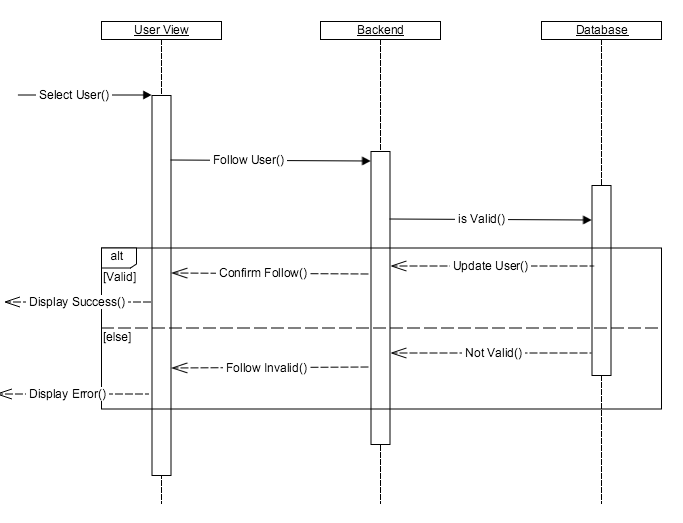
\includegraphics[width=\textwidth]{src/img/follow-user.png}
                \caption{Follow User Sequence Diagram} 
            \end{figure}

            From Profile view, the user selects follow. The request to follow is
            sent to the backend. The backend polls the database to verify that
            the request is valid. If the request is valid the database updates
            the users and returns. The backend then confirms the follow to
            Profile view. Profile view displays a success message to the user.
            If the request is not valid, the database returns an error to the
            backend. The backend serves an invalid response to Profile view.
            Profile view displays an error message to the user. 

        \subsubsection{Flag Post}
            \begin{figure}[H]
                \centering
                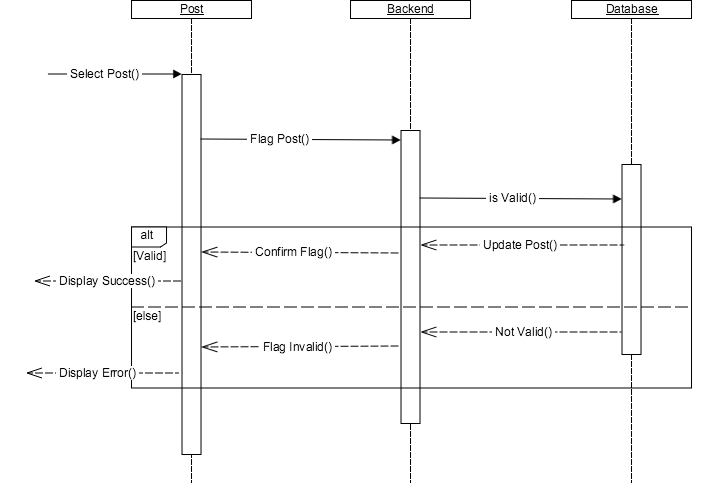
\includegraphics[width=\textwidth]{src/img/flag-post.png}
                \caption{Flag Post Sequence Diagram} 
            \end{figure}

            After a post has been selected by a user, they then choose to flag
            the post if it is offensive. The request is sent to the backend via
            a REST post. The backend polls the database to determine if the post
            is able to be flagged by that user. If the request is valid the
            database updates the post and returns success to the backend. The
            backend confirms the action of flagging to the selected post. A
            success message is then displayed to the user. If the request to
            flag is invalid, the database returns an error. The backend serves
            the post with an error, and the user is notified that the action was
            not valid. 

        \subsubsection{Create Account}
            \begin{figure}[H]
                \centering
                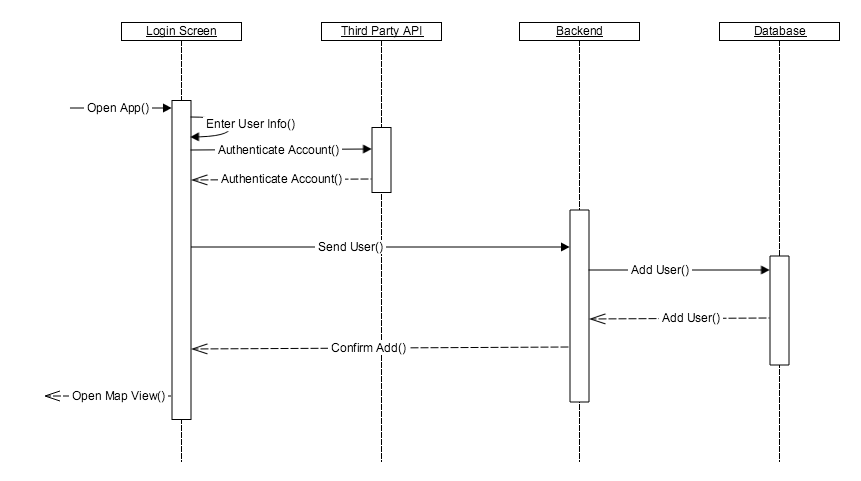
\includegraphics[width=\textwidth]{src/img/create-account.png}
                \caption{Create Account Sequence Diagram} 
            \end{figure}

            When the app is opened for the first time by a user, the user will
            be prompted to enter a username and to verify with a third party
            account. A third party API will then be sent an authentication
            request. Upon return of authentication of the account, the backend
            will be sent the new user information. The backend will poll the
            database to add the new user. The database will return success once
            the user is saved. The backend then serves the app with a success,
            and Map view is launched for the user.
